    % File: 2_co_so_ly_thuyet/2.3_chuan_giao_tiep.tex

    \subsection{Chuẩn giao tiếp AMBA AXI4}
    AMBA (Advanced Microcontroller Bus Architecture) là tiêu chuẩn kết nối trên chip (On-Chip Interconnect) phổ biến nhất hiện nay, được phát triển bởi ARM. Trong đó, giao thức AXI (Advanced eXtensible Interface) là chuẩn giao tiếp hiệu năng cao, được thiết kế cho các hệ thống SoC yêu cầu băng thông lớn và độ trễ thấp.

    Phiên bản AXI4 (được giới thiệu trong AMBA 4.0) hỗ trợ các tính năng vượt trội so với các thế hệ trước:
    \begin{itemize}
        \item Tách biệt hoàn toàn pha địa chỉ/điều khiển và pha dữ liệu.
        \item Hỗ trợ giao dịch dữ liệu không thẳng hàng (Unaligned data transfers).
        \item Cho phép phát hành nhiều địa chỉ chờ (Outstanding addresses) trước khi dữ liệu hoàn tất.
        \item Hỗ trợ hoàn thành giao dịch không theo thứ tự (Out-of-order completion) thông qua ID.
    \end{itemize}

    \begin{figure}[H]
        \centering
        \includegraphics[width=0.5\linewidth]{2_co_so_ly_thuyet/image/axi.png} 
        \caption{a. Tổng quan giao thức AXI4}
        \label{fig:axi_channels}
    \end{figure}

    \begin{figure}[H]
        \centering
        \includegraphics[width=0.9\linewidth]{2_co_so_ly_thuyet/image/axi2.png} 
        \caption{b. Tổng quan giao thức AXI4}
        \label{fig:axi_channels}
    \end{figure}



    \subsubsection{Kiến trúc 5 kênh độc lập (Channel Architecture)}
    AXI chia nhỏ một giao dịch truyền thông thành 5 kênh riêng biệt hoạt động song song. Kiến trúc này cho phép đường truyền dữ liệu hai chiều (Full-duplex), nghĩa là Master có thể ghi dữ liệu vào Slave trong khi đang đọc dữ liệu từ Slave khác.

    \begin{figure}[H]
        \centering
        \includegraphics[width=0.9\linewidth]{2_co_so_ly_thuyet/image/axichannel.png} 
        \caption{Mô hình 5 kênh giao tiếp của AXI4}
        \label{fig:axi_channels}
    \end{figure}

    Năm kênh tín hiệu bao gồm:
    \begin{enumerate}
        \item \textbf{Write Address Channel (AW):} Master gửi địa chỉ bắt đầu và thông tin điều khiển (loại burst, độ dài) cho giao dịch ghi. Các tín hiệu bắt đầu bằng \texttt{AW...} (ví dụ: \texttt{AWADDR}, \texttt{AWVALID}).
        \item \textbf{Write Data Channel (W):} Master truyền dữ liệu thực tế tới Slave. Kênh này hỗ trợ tín hiệu \texttt{WSTRB} (Strobe) để đánh dấu các byte hợp lệ trong một word (hỗ trợ ghi từng byte). Các tín hiệu bắt đầu bằng \texttt{W...}.
        \item \textbf{Write Response Channel (B):} Slave gửi phản hồi trạng thái (OKAY, ERROR) cho Master sau khi toàn bộ dữ liệu đã được ghi thành công. Tín hiệu bắt đầu bằng \texttt{B...}.
        \item \textbf{Read Address Channel (AR):} Master gửi địa chỉ bắt đầu cho giao dịch đọc. Tín hiệu bắt đầu bằng \texttt{AR...}.
        \item \textbf{Read Data Channel (R):} Slave trả về dữ liệu yêu cầu cùng với trạng thái đọc. Tín hiệu bắt đầu bằng \texttt{R...}.
    \end{enumerate}

    \subsubsection{Cơ chế bắt tay (Handshake Mechanism)}
    Toàn bộ 5 kênh AXI đều sử dụng chung một cơ chế bắt tay hai chiều \texttt{VALID/READY} để điều khiển luồng dữ liệu:
    \begin{itemize}
        \item \textbf{VALID (từ Bên gửi):} Báo hiệu rằng dữ liệu hoặc địa chỉ trên đường truyền đã hợp lệ và ổn định.
        \item \textbf{READY (từ Bên nhận):} Báo hiệu rằng bên nhận đã sẵn sàng chấp nhận dữ liệu mới.
    \end{itemize}

    \begin{figure}[H]
        \centering
        \includegraphics[width=0.9\linewidth]{2_co_so_ly_thuyet/image/battay.png} 
        \caption{Cơ chế bắt tay VALID/READY trong AXI}
        \label{fig:axi_handshake}
    \end{figure}

    Giao dịch chỉ thực sự diễn ra tại cạnh dương của xung nhịp khi và chỉ khi cả \texttt{VALID} và \texttt{READY} đều ở mức cao (High). Cơ chế này cho phép bên nhận có thể "kìm" (back-pressure) bên gửi nếu bộ đệm bị đầy, hoặc bên gửi có thể đợi chuẩn bị dữ liệu xong mới phát tín hiệu.

    Dựa trên cơ chế bắt tay này, chuẩn AXI định nghĩa hai cấp độ truyền tải dữ liệu cần phân biệt rõ:
    \begin{itemize}
        \item \textbf{Transfer (hoặc Beat):} Là một lần trao đổi dữ liệu đơn lẻ thành công (một lần bắt tay VALID/READY = 1). Trong một chuỗi dữ liệu (Burst), mỗi nhịp truyền một gói tin (ví dụ 32-bit) được gọi là một Transfer.
        
        \begin{figure}[H]
            \centering
            \includegraphics[width=0.9\linewidth]{2_co_so_ly_thuyet/image/transfer.png} 
            \caption{Minh họa một Transfer trong AXI}
            \label{fig:axi_handshake}
        \end{figure}

        \item \textbf{Transaction (Giao dịch):} Là một hoạt động đọc hoặc ghi hoàn chỉnh. Một Transaction bao gồm toàn bộ quá trình: gửi địa chỉ (Address Phase), truyền một hoặc nhiều dữ liệu (Data Phase - gồm nhiều Transfers) và nhận phản hồi (Response Phase).
        \begin{figure}[H]
            \centering
            \includegraphics[width=0.9\linewidth]{2_co_so_ly_thuyet/image/transaction.png} 
            \caption{Minh họa một Transaction trong AXI}
            \label{fig:axi_handshake}
        \end{figure}

    \end{itemize}

    % --- ĐOẠN BỔ SUNG VÀO SAU PHẦN TRANSFER/TRANSACTION ---% --- THAY THẾ CHO MỤC QUY TRÌNH GIAO DỊCH CŨ ---

    \subsubsection{Quy trình thực hiện giao dịch chi tiết (Transaction Steps)}
    Để đảm bảo toàn vẹn dữ liệu, chuẩn AXI quy định chặt chẽ về hướng đi của tín hiệu và trình tự bắt tay giữa Master và Slave. Dưới đây là mô tả chi tiết các tín hiệu tham gia vào hai loại giao dịch cơ bản.

    \textbf{1. Giao dịch Ghi (Write Transaction)} \\
    Quá trình ghi dữ liệu diễn ra qua 3 pha, sử dụng các kênh AW, W và B.

    \begin{figure}[H]
        \centering
        \includegraphics[width=0.9\linewidth]{2_co_so_ly_thuyet/image/write.png} 
        \caption{Giản đồ tín hiệu chi tiết của giao dịch Ghi}
        \label{fig:axi_write_trans}
    \end{figure}

    \begin{itemize}
        \item \textbf{Pha địa chỉ (Write Address Channel):}
        \begin{itemize}
            \item[] \textbf{Master $\rightarrow$ Slave:} Master đặt địa chỉ lên bus \texttt{AWADDR} và các thông tin điều khiển (Burst type, length) lên \texttt{AWLEN}, \texttt{AWSIZE}... sau đó xác lập tín hiệu \texttt{AWVALID = 1}.
            \item[] \textbf{Slave $\rightarrow$ Master:} Khi Slave sẵn sàng nhận địa chỉ, nó bật \texttt{AWREADY = 1}. Giao dịch địa chỉ hoàn tất.
        \end{itemize}
        
        \item \textbf{Pha dữ liệu (Write Data Channel):}
        \begin{itemize}
            \item[] \textbf{Master $\rightarrow$ Slave:} Master đưa dữ liệu lên bus \texttt{WDATA}. Nếu đây là gói cuối cùng trong Burst, Master bật tín hiệu \texttt{WLAST = 1}. Đồng thời, Master xác lập \texttt{WVALID = 1}.
            \item[] \textbf{Slave $\rightarrow$ Master:} Slave bật \texttt{WREADY = 1} để báo hiệu đã nhận gói dữ liệu đó. Quá trình lặp lại cho đến hết Burst.
        \end{itemize}

        \item \textbf{Pha phản hồi (Write Response Channel):}
        \begin{itemize}
            \item[] \textbf{Slave $\rightarrow$ Master:} Sau khi nhận đủ dữ liệu và hoàn tất việc ghi vào bộ nhớ, Slave gửi trạng thái (ví dụ: OKAY) qua bus \texttt{BRESP} và xác lập \texttt{BVALID = 1}.
            \item[] \textbf{Master $\rightarrow$ Slave:} Master xác nhận đã nhận được phản hồi bằng cách bật \texttt{BREADY = 1}. Kết thúc giao dịch.
        \end{itemize}
    \end{itemize}

    \textbf{2. Giao dịch Đọc (Read Transaction)} \\
    Quá trình đọc dữ liệu diễn ra qua 2 pha, sử dụng kênh AR và R.

    \begin{figure}[H]
        \centering
        \includegraphics[width=0.9\linewidth]{2_co_so_ly_thuyet/image/read.png} 
        \caption{Giản đồ tín hiệu chi tiết của giao dịch Đọc}
        \label{fig:axi_read_trans}
    \end{figure}

    \begin{itemize}
        \item \textbf{Pha địa chỉ (Read Address Channel):}
        \begin{itemize}
            \item[] \textbf{Master $\rightarrow$ Slave:} Master đặt địa chỉ cần đọc lên bus \texttt{ARADDR} cùng các tham số điều khiển, sau đó bật \texttt{ARVALID = 1}.
            \item[] \textbf{Slave $\rightarrow$ Master:} Slave chấp nhận địa chỉ bằng cách bật \texttt{ARREADY = 1}.
        \end{itemize}

        \item \textbf{Pha dữ liệu (Read Data Channel):}
        \begin{itemize}
            \item[] \textbf{Slave $\rightarrow$ Master:} Slave truy xuất dữ liệu và đưa lên bus \texttt{RDATA}. Nếu thành công, Slave gửi kèm trạng thái OKAY trên bus \texttt{RRESP}. Tại gói dữ liệu cuối cùng, Slave bật \texttt{RLAST = 1}. Tín hiệu \texttt{RVALID = 1} được xác lập khi dữ liệu trên bus là hợp lệ.
            \item[] \textbf{Master $\rightarrow$ Slave:} Master nhận dữ liệu bằng cách bật \texttt{RREADY = 1}.
        \end{itemize}
    \end{itemize}
    
    % --- HẾT PHẦN BỔ SUNG ---


    \subsubsection{Cấu trúc giao dịch Burst (Burst Transaction)}
    AXI là giao thức dựa trên Burst, nghĩa là chỉ cần gửi một địa chỉ khởi đầu, Master có thể truyền liên tiếp một chuỗi dữ liệu (tức là thực hiện một Transaction gồm nhiều Transfers). Các tham số chính điều khiển Burst bao gồm:

    \begin{itemize}
        \item \textbf{Burst Length (AxLEN):} Số lượng gói dữ liệu (beat/transfer) trong một burst. AXI4 hỗ trợ lên đến 256 beat cho kiểu INCR.
        \item \textbf{Burst Size (AxSIZE):} Số byte trong mỗi beat (ví dụ: 4 bytes cho hệ thống 32-bit).
        \item \textbf{Burst Type (AxBURST):} Xác định cách tính địa chỉ cho các beat tiếp theo:
        \begin{itemize}
            \item[] \textit{FIXED:} Địa chỉ giữ nguyên (dùng cho FIFO).
            \item[] \textit{INCR (Incrementing):} Địa chỉ tăng dần (dùng cho RAM). Đây là kiểu phổ biến nhất.
            \item[] \textit{WRAP:} Địa chỉ tăng đến giới hạn biên rồi quay vòng (dùng cho Cache Line fill).
        \end{itemize}
    \end{itemize}

    \subsubsection{Các biến thể giao thức trong thiết kế}
    Trong phiên bản AXI4, chuẩn AMBA định nghĩa thêm các biến thể rút gọn để phù hợp với từng mục đích sử dụng cụ thể:

    \textbf{1. Giao thức AXI4-Lite (AXI-Lite)} \\
    AXI4-Lite là một phiên bản rút gọn của AXI4, được thiết kế cho các giao tiếp điều khiển đơn giản, không yêu cầu truyền dữ liệu tốc độ cao (Burst transfer). Đặc điểm chính của AXI4-Lite bao gồm:
    \begin{itemize}
        \item Mỗi giao dịch chỉ truyền một gói dữ liệu đơn lẻ (Burst length = 1).
        \item Dữ liệu thường có độ rộng 32-bit hoặc 64-bit cố định.
        \item Đơn giản hóa logic điều khiển, giảm diện tích phần cứng.
    \end{itemize}
    Nhờ sự đơn giản này, AXI4-Lite thường được sử dụng làm giao diện cấu hình cho các thanh ghi điều khiển (Control Registers) bên trong các khối IP (Intellectual Property).

    \textbf{2. Giao thức AXI4-Stream (AXI-Stream)} \\
    AXI4-Stream được thiết kế chuyên biệt cho việc truyền tải các luồng dữ liệu liên tục tốc độ cao (Streaming data) mà không cần sử dụng địa chỉ. Khác với AXI4-Lite hay AXI4-Full (Memory Mapped), AXI4-Stream chỉ tập trung vào việc đẩy dữ liệu từ nguồn (Master) đến đích (Slave) nhanh nhất có thể.
    \begin{itemize}
        \item Không có kênh địa chỉ (Address Channel), giảm đáng kể số lượng dây tín hiệu.
        \item Hỗ trợ truyền dữ liệu liên tục không giới hạn độ dài Burst.
        \item Thích hợp cho dữ liệu video, âm thanh hoặc dữ liệu mạng nơ-ron (Feature maps).
    \end{itemize}

    \subsubsection{Áp dụng trong hệ thống đề tài}
    Trong khuôn khổ đồ án thiết kế SoC RISC-V tích hợp EdgeAI này, nhóm thực hiện áp dụng kết hợp cả hai chuẩn giao tiếp trên để tối ưu hóa hiệu năng và tài nguyên:

    \begin{itemize}
        \item \textbf{Sử dụng AXI4-Lite:} Đóng vai trò là kênh điều khiển (Control Plane). Vi xử lý PicoRV32 (Master) sẽ sử dụng AXI4-Lite để ghi vào các thanh ghi cấu hình của khối ngoại vi, khối Accelerator và DMA, thiết lập các thông số như kích thước ảnh, địa chỉ bộ nhớ và tín hiệu bắt đầu (Start).
        \item \textbf{Sử dụng AXI4-Stream:} Đóng vai trò là kênh dữ liệu (Data Plane). Dữ liệu hình ảnh từ Camera và các ma trận trọng số (Weights) sẽ được truyền trực tiếp từ DMA vào khối Accelerator thông qua AXI4-Stream. Việc loại bỏ overhead của kênh địa chỉ giúp tối đa hóa băng thông xử lý cho mạng CNN.
    \end{itemize}

    %%%%%%%%%%%%%%%%%%%%%%%%%%%%%%%%%%%%%%%%%%%%%
    \subsection{Giao thức truyền thông UART}

    UART (Universal Asynchronous Receiver-Transmitter) là một vi mạch phần cứng dùng để truyền tải dữ liệu nối tiếp giữa hai thiết bị. Khác với các giao thức đồng bộ như SPI hay I2C, UART hoạt động theo cơ chế bất đồng bộ (Asynchronous), nghĩa là không cần tín hiệu xung nhịp (Clock) chung để đồng bộ hóa việc truyền nhận giữa bên gửi và bên nhận.

    Trong các thiết kế SoC, UART thường được tích hợp như một khối ngoại vi (Peripheral) để phục vụ việc gỡ lỗi (Debug), in log hệ thống hoặc giao tiếp với máy tính.

    \subsubsection{Nguyên lý hoạt động}
    Giao thức UART truyền dữ liệu trên hai dây tín hiệu riêng biệt:
    \begin{itemize}
        \item \textbf{TX (Transmit):} Chân truyền dữ liệu đi.
        \item \textbf{RX (Receive):} Chân nhận dữ liệu về.
    \end{itemize}
    Để giao tiếp thành công, chân TX của thiết bị này phải được nối với chân RX của thiết bị kia và ngược lại. Quá trình truyền tin diễn ra bằng cách chuyển đổi dữ liệu song song (Parallel data) từ bus hệ thống thành luồng dữ liệu nối tiếp (Serial bit stream) tại phía phát, và khôi phục lại thành song song tại phía thu.
    
    \begin{figure}[H]
        \centering
        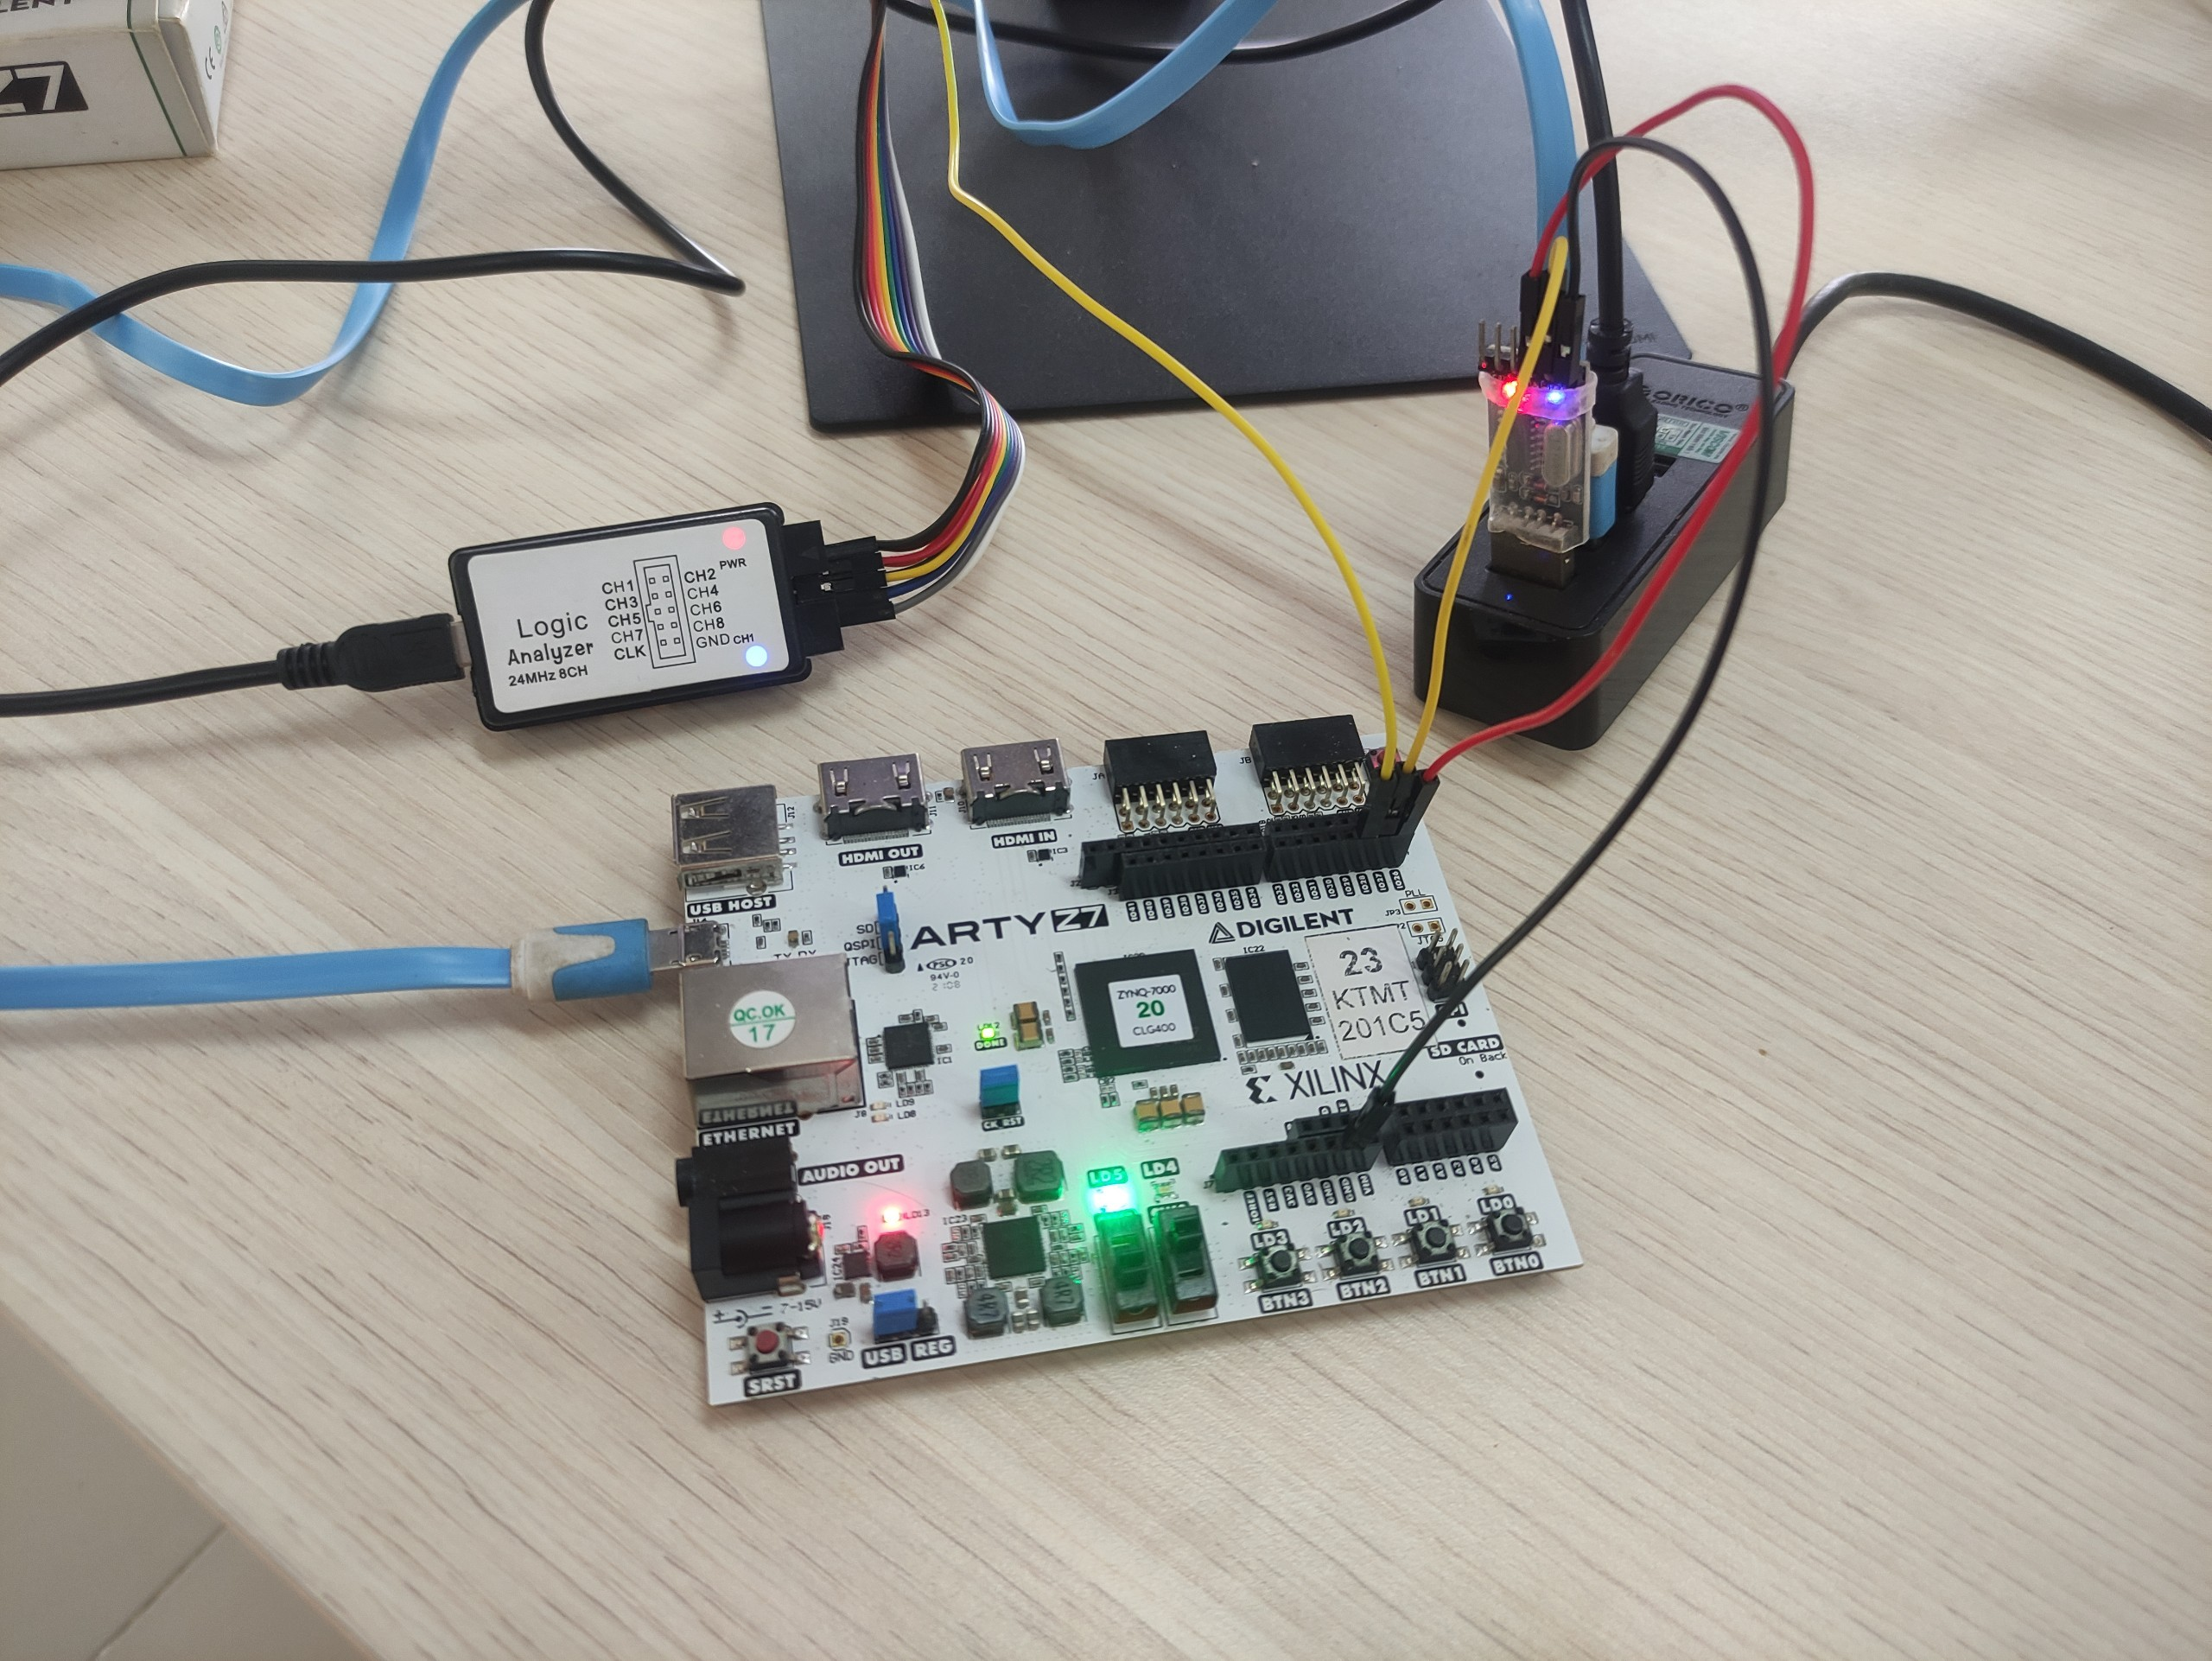
\includegraphics[width=0.9\linewidth]{2_co_so_ly_thuyet/image/uart.png} 
        \caption{Minh họa chân kết nối truyền nhận dữ liệu UART}
        \label{fig:uart_connection}
    \end{figure}

    \begin{figure}[H]
        \centering
        \includegraphics[width=0.8\linewidth]{2_co_so_ly_thuyet/image/uart2.png} 
        \caption{Chuyển đổi dữ liệu song song thành nối tiếp và ngược lại trong UART}
        \label{fig:uart_connection}
    \end{figure}



    \subsubsection{Cấu trúc khung dữ liệu (Data Frame)}
    Do không có xung nhịp đồng bộ, UART sử dụng các bit điều khiển đặc biệt để đánh dấu điểm bắt đầu và kết thúc của một gói tin. Một khung dữ liệu chuẩn bao gồm các thành phần sau:



    \begin{enumerate}
        \item \textbf{Trạng thái nghỉ (Idle State):} Khi không có dữ liệu truyền, đường truyền luôn được giữ ở mức điện áp cao (Logic 1).
        \item \textbf{Start Bit:} Để bắt đầu một phiên truyền, thiết bị phát sẽ kéo đường truyền từ mức cao xuống mức thấp (Logic 0) trong một chu kỳ bit. Bên thu phát hiện cạnh xuống này để bắt đầu quá trình đồng bộ.
        \item \textbf{Data Bits:} Chứa thông tin thực tế cần truyền, thường có độ dài từ 5 đến 9 bit (phổ biến nhất là 8 bit). Theo quy ước, bit có trọng số nhỏ nhất (LSB) được truyền đi trước.
        \item \textbf{Parity Bit (Tùy chọn):} Dùng để kiểm tra lỗi đơn giản. Bit này có thể được cấu hình là chẵn (Even), lẻ (Odd) hoặc không sử dụng (None). Nếu sử dụng, tổng số bit '1' trong gói dữ liệu (bao gồm cả parity) phải thỏa mãn quy tắc chẵn/lẻ đã thiết lập.
        \item \textbf{Stop Bit:} Đánh dấu kết thúc gói tin bằng cách kéo đường truyền về mức cao (Logic 1). Độ dài có thể là 1, 1.5, hoặc 2 bit thời gian. Stop bit đảm bảo đường truyền quay về trạng thái nghỉ để sẵn sàng cho Start bit tiếp theo.
    \end{enumerate}

    \begin{figure}[H]
        \centering
        \includegraphics[width=0.8\linewidth]{2_co_so_ly_thuyet/image/uart_frame.png} 
        \caption{Khung dữ liệu UART}
        \label{fig:uart_frame}
    \end{figure}

    \begin{figure}[H]
        \centering
        \includegraphics[width=0.8\linewidth]{2_co_so_ly_thuyet/image/uart_frame_example.png} 
        \caption{Ví dụ khung dữ liệu UART với 8bit dữ liệu, không parity và 1 stop bit}
        \label{fig:uart_frame}
    \end{figure}

    \subsubsection{Tốc độ Baud (Baud Rate)}
    Vì thiếu xung nhịp đồng bộ, hai thiết bị UART phải thống nhất trước một tốc độ truyền nhận, gọi là Baud Rate (đơn vị: bit/giây - bps).
    \begin{itemize}
        \item Bên phát sẽ đẩy từng bit dữ liệu ra đường truyền với chu kỳ $T = 1/BaudRate$.
        \item Bên thu sẽ lấy mẫu tín hiệu (sample) tại điểm giữa của mỗi chu kỳ bit dự kiến để đọc dữ liệu.
    \end{itemize}
    Theo khuyến cáo kỹ thuật, độ sai lệch tốc độ Baud giữa hai thiết bị không được vượt quá 10\% để đảm bảo dữ liệu được đọc chính xác. Các tốc độ phổ biến thường dùng là 9600, 19200, 115200 bps.


    \subsection{Giao thức truyền thông SPI}

SPI (Serial Peripheral Interface) là chuẩn giao tiếp nối tiếp đồng bộ tốc độ cao, hoạt động ở chế độ song công toàn phần (Full-duplex). Chuẩn này được Motorola giới thiệu vào giữa những năm 1980 và hiện nay đã trở thành tiêu chuẩn công nghiệp để kết nối vi xử lý với các thiết bị ngoại vi như cảm biến, bộ nhớ Flash (SPI Flash), màn hình LCD, hoặc bộ chuyển đổi ADC/DAC.

Khác với UART (bất đồng bộ) hay I2C (bán song công, tốc độ thấp), SPI sử dụng đường xung nhịp riêng biệt và kiến trúc Master-Slave chặt chẽ, cho phép đạt băng thông truyền tải rất cao (có thể lên tới hàng chục MHz).

\subsubsection{Cấu hình tín hiệu vật lý}
Một bus SPI tiêu chuẩn (4-wire mode) bao gồm 4 đường tín hiệu logic kết nối giữa Master và Slave.

% --- VỊ TRÍ CHÈN ẢNH 1: Sơ đồ kết nối Master-Slave ---
\begin{figure}[H]
    \centering
    % Bạn thay tên file ảnh vào dòng dưới
    \includegraphics[width=0.7\linewidth]{2_co_so_ly_thuyet/image/spiwrite.png} 
    \caption{Sơ đồ kết nối tín hiệu chuẩn 4 dây của SPI}
    \label{fig:spi_connection}
\end{figure}

Chức năng các chân tín hiệu bao gồm:
\begin{itemize}
    \item \textbf{SCLK (Serial Clock):} Tín hiệu xung nhịp do Master tạo ra. Toàn bộ quá trình truyền nhận dữ liệu được đồng bộ theo cạnh lên hoặc cạnh xuống của xung này. Slave không được phép tạo xung Clock.
    \item \textbf{MOSI (Master Out Slave In):} Đường truyền dữ liệu từ Master đến Slave.
    \item \textbf{MISO (Master In Slave Out):} Đường truyền dữ liệu từ Slave về Master. Nếu chỉ có Master gửi dữ liệu (ví dụ điều khiển LCD), chân này có thể bỏ qua.
    \item \textbf{CS/SS (Chip Select / Slave Select):} Tín hiệu chọn thiết bị, thường hoạt động ở mức thấp (Active Low). Master kéo chân này xuống 0V để bắt đầu giao dịch với một Slave cụ thể.
\end{itemize}

\subsubsection{Cơ chế hoạt động: Thanh ghi dịch (Shift Register)}
Cốt lõi của giao thức SPI là cấu trúc thanh ghi dịch vòng tròn (Circular Shift Register).

% --- VỊ TRÍ CHÈN ẢNH 2: Cơ chế thanh ghi dịch ---
\begin{figure}[H]
    \centering
    % Bạn thay tên file ảnh vào dòng dưới
    \includegraphics[width=0.9\linewidth]{2_co_so_ly_thuyet/image/spireg.png} 
    \caption{Cơ chế trao đổi dữ liệu dùng thanh ghi dịch trong SPI}
    \label{fig:spi_shift_register}
\end{figure}

Quá trình truyền nhận diễn ra như sau:
\begin{enumerate}
    \item Master và Slave mỗi bên đều có một thanh ghi dịch (thường là 8-bit hoặc 16-bit).
    \item Tại mỗi chu kỳ xung nhịp SCLK:
    \begin{itemize}
        \item 1 bit dữ liệu từ Master được đẩy ra đường MOSI và dịch vào thanh ghi của Slave.
        \item Đồng thời, 1 bit dữ liệu từ Slave được đẩy ra đường MISO và dịch vào thanh ghi của Master.
    \end{itemize}
    \item Sau $N$ chu kỳ xung nhịp (với $N$ là độ rộng dữ liệu), giá trị trong thanh ghi của Master và Slave được trao đổi hoàn toàn cho nhau.
    
\end{enumerate}

\subsubsection{Các chế độ hoạt động (Clock Polarity \& Phase)}
SPI định nghĩa 4 chế độ hoạt động (Modes) dựa trên trạng thái của xung Clock, được quy định bởi hai tham số:
\begin{itemize}
    \item \textbf{CPOL (Clock Polarity):} Trạng thái nghỉ của đường SCLK (0 hoặc 1).
    \item \textbf{CPHA (Clock Phase):} Cạnh lên hoặc xuống của xung dùng để lấy mẫu (Sample) và dùng để thay đổi dữ liệu (Shift).
\end{itemize}

% --- VỊ TRÍ CHÈN ẢNH 3: Giản đồ xung 4 Mode (Lấy từ file Analog Device) ---
% \begin{figure}[H]
%     \centering
%     % Bạn thay tên file ảnh vào dòng dưới
%     \includegraphics[width=0.9\linewidth]{2_co_so_ly_thuyet/image/spi_modes.png} 
%     \caption{Giản đồ thời gian của 4 chế độ hoạt động SPI (CPOL/CPHA)}
%     \label{fig:spi_modes}
% \end{figure}

\begin{figure}[H]
    \centering
    % Bạn thay tên file ảnh vào dòng dưới
    \includegraphics[width=1\linewidth]{2_co_so_ly_thuyet/image/spimode.png} 
    \caption{4 chế độ hoạt động của SPI(CPOL/CPHA)}
    \label{fig:spi_modes}
\end{figure}


\textit{Lưu ý:} Mode 0 và Mode 3 là hai cấu hình phổ biến nhất. Master và Slave phải được cấu hình cùng một Mode để giao tiếp thành công.

\begin{figure}[H]
    \centering
    % Bạn thay tên file ảnh vào dòng dưới
    \includegraphics[width=1\linewidth]{2_co_so_ly_thuyet/image/spimod0.png} 
    \caption{SPI MODE 0 (CPOL=0, CPHA=0), trạng thái SCLK ban đầu ở mức low, dữ liệu được lấy mẫu tại cạnh lên của SCLK và dịch ở cạnh xuống}
    \label{fig:spi_modes}
\end{figure}

\begin{figure}[H]
    \centering
    % Bạn thay tên file ảnh vào dòng dưới
    \includegraphics[width=1\linewidth]{2_co_so_ly_thuyet/image/spimode3.png} 
    \caption{SPI MODE 3 (CPOL=1, CPHA=1), trạng thái SCLK ban đầu ở mức high, dữ liệu được lấy mẫu tại cạnh lên của SCLK và dịch ở cạnh xuống}
    \label{fig:spi_modes}
\end{figure}

\subsubsection{Các mô hình kết nối đa thiết bị}
SPI cho phép một Master giao tiếp với nhiều Slave thông qua hai cấu hình chính:

\textbf{1. Cấu hình Slave độc lập (Independent Slaves):} \\
Master sử dụng các chân CS riêng biệt ($CS_1, CS_2, ...$) cho từng Slave. Đây là cấu hình phổ biến giúp tối ưu băng thông.

\begin{figure}[H]
    \centering
    % Bạn thay tên file ảnh vào dòng dưới
    \includegraphics[width=0.9\linewidth]{2_co_so_ly_thuyet/image/spisingle.png} 
    \caption{Cấu hình Slave độc lập trong SPI}
    \label{fig:spi_modes}
\end{figure}

\textbf{2. Cấu hình Chuỗi (Daisy Chain):} \\
Các Slave được nối tiếp nhau (MISO của Slave này nối vào MOSI của Slave kia). Dữ liệu đi qua chuỗi các thiết bị, giúp tiết kiệm chân điều khiển của Master nhưng làm giảm tốc độ truyền tổng thể.

\begin{figure}[H]
    \centering
    % Bạn thay tên file ảnh vào dòng dưới
    \includegraphics[width=0.9\linewidth]{2_co_so_ly_thuyet/image/spidaisy.png} 
    \caption{Cấu hình Chuỗi (Daisy Chain) trong SPI}
    \label{fig:spi_modes}
\end{figure}




    SPI có tốc độ truyền cao nhất so với UART và I2C, phần cứng đơn giản, hỗ trợ Full-duplex. Nhưng tốn nhiều dây tín hiệu, khoảng cách truyền ngắn, không có cơ chế xác nhận lỗi (ACK) như I2C.


    \subsection{Giao thức truyền thông OSPI (Octal SPI)}

    Mặc dù giao thức SPI truyền thống có ưu điểm về sự đơn giản, nhưng giới hạn về độ rộng băng thông (chỉ truyền 1 bit mỗi chu kỳ) trở thành nút thắt cổ chai đối với các ứng dụng hiện đại yêu cầu truy xuất dữ liệu lớn như EdgeAI. Để giải quyết vấn đề này, các biến thể mở rộng độ rộng bus dữ liệu đã lần lượt ra đời: từ Dual-SPI (2 đường dữ liệu), Quad-SPI (4 đường dữ liệu - QSPI) và bước tiến mới nhất là \textbf{OSPI (Octal SPI)}.

    OSPI (còn được gọi là xSPI theo chuẩn JEDEC JESD251) mở rộng giao tiếp lên \textbf{8 đường dữ liệu song song}, đồng thời tích hợp công nghệ \textbf{DDR (Double Data Rate)}. Đây là giải pháp tối ưu được lựa chọn trong đề tài để kết nối SoC RISC-V với các bộ nhớ ngoài tốc độ cao (như Octal Flash hoặc HyperRAM), đảm bảo khả năng nạp trọng số mạng nơ-ron (Weights) và dữ liệu hình ảnh với độ trễ thấp nhất.

    \subsubsection{Cấu hình tín hiệu vật lý}
    Để hỗ trợ truyền tải 8 bit song song, giao diện OSPI yêu cầu số lượng chân tín hiệu nhiều hơn so với chuẩn SPI 4 dây truyền thống. Các tín hiệu chính bao gồm:

    \begin{figure}[H]
        \centering
        % Bạn có thể chèn hình pinout của OSPI/HyperRAM vào đây
        \includegraphics[width=0.9\linewidth]{2_co_so_ly_thuyet/image/ospipinout.png} 
        \caption{Sơ đồ chân tín hiệu của giao diện OSPI/HyperBus}
        \label{fig:ospi_pinout}
    \end{figure}

    \begin{itemize}
        \item \textbf{CLK (Serial Clock):} Tín hiệu xung nhịp đồng bộ do Master cấp.
        \item \textbf{CS/SS (Chip Select):} Tín hiệu chọn chip (Active Low).
        \item \textbf{IO0 - IO7 (Data Lines):} 8 đường dữ liệu hai chiều (Bi-directional). Trong một chu kỳ xung nhịp, 8 bit có thể được truyền đi đồng thời (1 Byte).
        \item \textbf{DQS / DS (Data Strobe):} Đây là tín hiệu đặc biệt chỉ xuất hiện trên các chuẩn tốc độ cao (như OSPI và bộ nhớ DDR DRAM).
        \begin{itemize}
            \item[] DQS là tín hiệu hai chiều, được tạo ra bởi thiết bị đang \textit{phát} dữ liệu (Source Synchronous).
            \item[] Nó đóng vai trò như một xung nhịp tham chiếu đi kèm với dữ liệu, giúp bên thu xác định chính xác thời điểm lấy mẫu dữ liệu hợp lệ mà không bị ảnh hưởng bởi độ trễ đường truyền ở tần số cao.
        \end{itemize}
        \item \textbf{RWDS (Read Write Data Strobe):} Trong giao diện HyperRAM (một biến thể tương tự OSPI), chân này vừa đóng vai trò là DQS, vừa dùng để chỉ thị mặt nạ dữ liệu (Data Mask) khi ghi.
    \end{itemize}

    \subsubsection{Cơ chế truyền tải DDR (Double Data Rate)}
    Điểm đột phá về hiệu năng của OSPI so với các thế hệ trước (SPI/QSPI) nằm ở khả năng hỗ trợ chế độ \textbf{DDR} (còn gọi là DTR - Double Transfer Rate).

    \textbf{1. So sánh SDR và DDR:}
    \begin{itemize}
        \item \textbf{SDR (Single Data Rate):} Dữ liệu chỉ được truyền ở một \textbf{cạnh} của xung nhịp (thường là \textbf{cạnh lên}). Đây là cách hoạt động của SPI và QSPI truyền thống.
        \item \textbf{DDR (Double Data Rate):} Dữ liệu được truyền ở \textbf{cả cạnh lên và cạnh xuống} của xung nhịp.
    \end{itemize}
    
    \begin{figure}[H]
        \centering
        % Chèn hình giản đồ sóng DDR từ datasheet Winbond vào đây
        \includegraphics[width=0.9\linewidth]{2_co_so_ly_thuyet/image/ddrsdr.png} 
        \caption{Giản đồ thời gian truyền tải SDR: Dữ liệu thay đổi ở cạnh lênh, DDR: Dữ liệu thay đổi ở cả hai cạnh của xung nhịp}
        \label{fig:ospi_ddr_timing}
    \end{figure}
    
    \textbf{2. Hiệu năng tính toán:}
    Với giao diện 8 đường dữ liệu (IO0-IO7) hoạt động ở chế độ DDR:
    \begin{itemize}
        \item Tại \textbf{cạnh lên (Rising Edge)}: Truyền 8 bit.
        \item Tại \textbf{cạnh xuống (Falling Edge)}: Truyền 8 bit.
        \item \textbf{Tổng cộng:} 16 bit (2 Bytes) được truyền trong một chu kỳ xung nhịp (Clock Cycle).
    \end{itemize}

    Ví dụ: Với xung nhịp 200MHz, băng thông lý thuyết của OSPI DDR đạt: $200 \text{ MHz} \times 2 \text{ Bytes} = 400 \text{ MB/s}$. Tốc độ này nhanh gấp 8 lần so với QSPI thông thường (chạy SDR) và tiệm cận với các giao tiếp DRAM, đủ đáp ứng nhu cầu xử lý thời gian thực.

   

    \subsubsection{Cấu trúc giao dịch Octal-DDR}
    Một giao dịch OSPI điển hình (ví dụ đọc bộ nhớ Flash W35T51NW) diễn ra theo các pha, trong đó toàn bộ Command, Address và Data đều có thể được truyền trên 8 dây (Mode \textbf{8-8-8}, nghĩa là sử dụng toàn bộ 8 đường dữ liệu cho cả ba giai đoạn Command Phase, Address Phase và Data Phase):

    \begin{enumerate}
        \item \textbf{Command Phase:} Master gửi mã lệnh (8-bit hoặc 16-bit) trên 8 dây IO.
        \item \textbf{Address Phase:} Master gửi địa chỉ truy cập (32-bit hoặc 64-bit) trên 8 dây IO theo chế độ DDR.
        \item \textbf{Dummy Cycles:} Các chu kỳ chờ để bộ nhớ chuẩn bị dữ liệu. Số lượng chu kỳ này có thể cấu hình được để phù hợp với tần số hoạt động.
        \item \textbf{Data Phase:} Dữ liệu được truyền đi (Write) hoặc nhận về (Read) trên cả 8 dây IO tại cả hai \textbf{cạnh} xung nhịp, đồng bộ với tín hiệu DQS.
    \end{enumerate}


    \begin{figure}[H]
        \centering
        % Chèn hình giản đồ sóng DDR từ datasheet Winbond vào đây
        \includegraphics[width=0.9\linewidth]{2_co_so_ly_thuyet/image/ospitransaction.png} 
        \caption{Giản đồ thời gian giao dịch OSPI DDR: Command, Address và Data truyền trên 8 dây IO}
        \label{fig:ospi_ddr_timing}
    \end{figure}

    \subsubsection{Ưu điểm trong ứng dụng SoC IoT}
    \begin{itemize}
        \item \textbf{Tốc độ cao:} Băng thông lớn giúp giảm thời gian nạp Bootloader và nạp trọng số mạng nơ-ron (Weights) vào Accelerator.
        \item \textbf{Số lượng chân ít:} So với các giao tiếp bộ nhớ song song truyền thống (Parallel Flash/SRAM) cần 30-40 chân, OSPI chỉ cần khoảng 12 chân, giúp tiết kiệm diện tích SoC.
    \end{itemize}




    \subsection{Giao thức truyền thông I2C (Inter-Integrated Circuit)}

    I2C (Inter-Integrated Circuit), thường được viết là $I^2C$, là một giao thức truyền thông nối tiếp đồng bộ, hoạt động ở chế độ bán song công (Half-duplex). Chuẩn này được Philips Semiconductors (nay là NXP Semiconductors) phát triển vào đầu những năm 1980 với mục đích đơn giản hóa việc kết nối giữa vi xử lý trung tâm và các linh kiện ngoại vi tốc độ thấp trên cùng một bo mạch (như EEPROM, cảm biến nhiệt độ, RTC).

    Khác với SPI (cần 4 dây) hay UART (cần 2 dây riêng biệt cho TX/RX), I2C chỉ sử dụng duy nhất \textbf{2 đường dây tín hiệu} để kết nối nhiều thiết bị (Multi-master, Multi-slave), giúp tiết kiệm đáng kể số lượng chân IO và diện tích đi dây trên PCB.

    \subsubsection{Cấu hình vật lý và Nguyên lý  Open-Drain}
    Mạng lưới I2C bao gồm hai đường tín hiệu hai chiều (Bidirectional):
    \begin{itemize}
        \item \textbf{SDA (Serial Data):} Đường truyền dữ liệu.
        \item \textbf{SCL (Serial Clock):} Đường xung nhịp đồng bộ (thường do Master tạo ra).
    \end{itemize}

    \begin{figure}[H]
        \centering
        % Placeholder cho sơ đồ kết nối vật lý
        \includegraphics[width=0.9\linewidth]{2_co_so_ly_thuyet/image/i2c.png} 
        \caption{Sơ đồ kết nối vật lý I2C}
        \label{fig:i2c_physical}
    \end{figure}

    Đặc điểm phần cứng quan trọng nhất của I2C là cấu trúc ngõ ra \textbf{(Open-Drain)} 
    \begin{itemize}
        \item Các thiết bị Master và Slave chỉ có thể kéo đường dây xuống mức thấp (Logic 0). Chúng không thể chủ động đẩy đường dây lên mức cao (Logic 1).
        \item Để tạo ra mức Logic 1, cần phải có các \textbf{điện trở kéo lên (Pull-up resistors)} nối từ đường SDA/SCL lên nguồn VCC.
        \item Cơ chế này cho phép thực hiện kỹ thuật "Wired-AND", giúp tránh hiện tượng ngắn mạch khi hai thiết bị cùng lái bus và hỗ trợ tính năng \textit{Clock Stretching} (kéo dãn xung nhịp).
    \end{itemize}

    \begin{figure}[H]
        \centering
        % Placeholder cho sơ đồ kết nối vật lý
        \includegraphics[width=0.9\linewidth]{2_co_so_ly_thuyet/image/i2c_pullup.png} 
        \caption{a. Điện trở kéo lên (Pull-up Resistors)}
        \label{fig:i2c_physical}
    \end{figure}

    \begin{figure}[H]
        \centering
        % Placeholder cho sơ đồ kết nối vật lý
        \includegraphics[width=0.9\linewidth]{2_co_so_ly_thuyet/image/i2c_pullup2.png} 
        \caption{b. Điện trở kéo lên (Pull-up Resistors)}
        \label{fig:i2c_physical}
    \end{figure}

    \subsubsection{Giao thức truyền dữ liệu}
    Quá trình truyền tin trên I2C tuân thủ chặt chẽ các quy tắc về định dạng khung (Frame format) và trạng thái bit.

    \begin{figure}[H]
        \centering
        % Placeholder cho sơ đồ kết nối vật lý
        \includegraphics[width=1\linewidth]{2_co_so_ly_thuyet/image/i2c_frame.png} 
        \caption{Cấu trúc khung truyền dữ liệu I2C}
        \label{fig:i2c_frame}
    \end{figure}

    \textbf{1. Điều kiện Bắt đầu (Start) và Kết thúc (Stop):}
    Thông thường, dữ liệu chỉ được phép thay đổi khi SCL ở mức Thấp. Tuy nhiên, có hai ngoại lệ đặc biệt dùng để báo hiệu trạng thái bus:
    \begin{itemize}
        \item \textbf{Start Condition (S):} SDA chuyển từ Cao xuống Thấp trong khi SCL đang ở mức Cao. Báo hiệu bắt đầu một giao dịch.
        \item \textbf{Stop Condition (P):} SDA chuyển từ Thấp lên Cao trong khi SCL đang ở mức Cao. Báo hiệu kết thúc giao dịch.
    \end{itemize}

    \begin{figure}[H]
        \centering
        % Placeholder cho giản đồ Start/Stop
        \includegraphics[width=\linewidth]{2_co_so_ly_thuyet/image/i2c_startstop.png} 
        \caption{Giản đồ thời gian của điều kiện Start và Stop trong I2C}
        \label{fig:i2c_start_stop}
    \end{figure}

    \textbf{2. Định dạng địa chỉ và Bit R/W:}
    Mỗi thiết bị Slave trên bus I2C được định danh bởi một địa chỉ duy nhất (thường là 7-bit, hỗ trợ tối đa 128 địa chỉ).
    \begin{itemize}
        \item Sau tín hiệu Start, Master gửi 1 byte đầu tiên bao gồm: \textbf{7 bit địa chỉ} của Slave + \textbf{1 bit R/W} (Read/Write).
        \item Nếu Bit R/W = 0: Master muốn Ghi dữ liệu vào Slave.
        \item Nếu Bit R/W = 1: Master muốn Đọc dữ liệu từ Slave.
    \end{itemize}

    \textbf{3. Cơ chế xác nhận (ACK/NACK):}
    Sau mỗi byte dữ liệu (8 bit) được truyền đi, bên nhận (Receiver) bắt buộc phải phản hồi bằng một bit xác nhận (Acknowledge bit) trong chu kỳ xung nhịp thứ 9.
    \begin{itemize}
        \item \textbf{ACK (Logic 0):} Bên nhận kéo đường SDA xuống thấp, báo hiệu đã nhận byte thành công và sẵn sàng nhận tiếp.
        \item \textbf{NACK (Logic 1):} Bên nhận để đường SDA ở mức cao (do điện trở pull-up). Báo hiệu lỗi, hoặc Slave đang bận, hoặc kết thúc quá trình đọc.
    \end{itemize}

    \begin{figure}[H]
        \centering
        % Placeholder cho khung dữ liệu I2C
        \includegraphics[width=1\linewidth]{2_co_so_ly_thuyet/image/i2c_frame2.png} 
        \caption{Cấu trúc một khung truyền dữ liệu I2C cơ bản}
        \label{fig:i2c_frame}
    \end{figure}

    \subsubsection{Các tốc độ hoạt động}
    Giao thức I2C hỗ trợ nhiều cấp độ tốc độ khác nhau tùy thuộc vào ứng dụng:
    \begin{itemize}
        \item \textbf{Standard Mode (Sm):} Tốc độ lên đến 100 kbps (phổ biến nhất).
        \item \textbf{Fast Mode (Fm):} Tốc độ lên đến 400 kbps.
        \item \textbf{Fast Mode Plus (Fm+):} Tốc độ lên đến 1 Mbps.
        \item \textbf{High Speed Mode (Hs):} Tốc độ lên đến 3.4 Mbps.
    \end{itemize}
    Trong phạm vi đồ án này, các ngoại vi cảm biến và cấu hình Camera thường sử dụng Standard Mode. 

    \subsubsection{Đánh giá ưu nhược điểm}
            I2C giúp tiết kiệm chân phần cứng (chỉ cần 2 dây cho hàng trăm thiết bị).
            Có cơ chế xác nhận lỗi (ACK) giúp truyền tin tin cậy.
            Hỗ trợ đa chủ (Multi-master).

            Nhưng về tốc độ chậm hơn nhiều so với SPI và OSPI.
            Cấu trúc cực máng hở tiêu thụ năng lượng qua điện trở kéo lên.
            Logic điều khiển phức tạp hơn SPI do phải phát hiện Start/Stop/ACK.


\subsection{Giao diện Camera song song (DVP Interface)}

Trong các hệ thống nhúng và FPGA tầm trung, Digital Video Port (DVP) là chuẩn giao tiếp song song phổ biến nhất để kết nối với cảm biến hình ảnh, điển hình như module OV5640 được sử dụng trong đồ án này. Khác với chuẩn MIPI CSI-2 yêu cầu phần cứng vật lý (PHY) tốc độ cao và logic giải mã phức tạp, DVP hoạt động dựa trên cơ chế truyền dữ liệu song song đồng bộ nguồn (Source Synchronous), giúp đơn giản hóa đáng kể việc thiết kế bộ điều khiển trên FPGA.

\subsubsection{Đặc tả tín hiệu và Cơ chế vật lý}
Về mặt vật lý, giao diện DVP thiết lập một kênh truyền dữ liệu một chiều từ Camera sang FPGA. Tín hiệu xung nhịp điểm ảnh \textbf{PCLK} (Pixel Clock) đóng vai trò là nhịp đập trung tâm của hệ thống; toàn bộ dữ liệu trên bus song song chỉ được xác định là hợp lệ tại cạnh tích cực (thường là cạnh lên) của xung PCLK. Để đồng bộ hóa luồng dữ liệu này thành các bức ảnh hoàn chỉnh, DVP sử dụng hai tín hiệu điều khiển quan trọng là \textbf{VSYNC} (Vertical Sync) và \textbf{HREF} (Horizontal Reference).

\begin{figure}[H]
    \centering
    \includegraphics[width=0.9\linewidth]{2_co_so_ly_thuyet/image/cameradvp.png} 
    \caption{Sơ đồ kết nối tín hiệu vật lý giữa Camera DVP và FPGA }
    \label{fig:dvp_interface}
\end{figure}

Tín hiệu VSYNC xác định thời điểm bắt đầu của một khung hình mới. Khi VSYNC được kích hoạt (thường là một xung mức cao ngắn), bộ thu phía FPGA sẽ nhận biết để đặt lại các con trỏ bộ nhớ về vị trí gốc $(0,0)$. Trong khi đó, tín hiệu HREF chịu trách nhiệm định khung cho từng dòng quét ngang. Dữ liệu trên bus \textbf{DATA[9:2]} chỉ được coi là điểm ảnh hợp lệ khi HREF ở mức cao. Ngược lại, khi HREF ở mức thấp, hệ thống hiểu rằng Camera đang trong thời gian nghỉ (Blanking time) để chuẩn bị cho dòng quét tiếp theo. Ngoài ra, FPGA cần cấp một xung nhịp hệ thống \textbf{XCLK} (thường là 24MHz) để cảm biến có thể hoạt động và tạo ra PCLK nội bộ.

\subsubsection{Định dạng dữ liệu RGB565 trên bus 8-bit}
Một thách thức kỹ thuật khi sử dụng cảm biến OV5640 ở chế độ DVP là sự chênh lệch về độ rộng dữ liệu. Mặc dù điểm ảnh màu RGB565 yêu cầu 16 bit để biểu diễn (5 bit Red, 6 bit Green, 5 bit Blue), nhưng để tiết kiệm tài nguyên chân I/O trên module Camera, bus dữ liệu thường chỉ được cấu hình sử dụng 8 dây (D[9:2]).

Do đó, một điểm ảnh 16-bit buộc phải được truyền tải trong hai chu kỳ xung nhịp PCLK liên tiếp. Chu kỳ đầu tiên truyền byte cao (bao gồm phần màu Đỏ và 3 bit cao của màu Lục), và chu kỳ thứ hai truyền byte thấp (bao gồm 3 bit thấp của màu Lục và phần màu Lam). Cơ chế này đòi hỏi bộ điều khiển trên FPGA phải được thiết kế logic ghép kênh (Byte Packing) để tái tạo lại giá trị pixel chính xác trước khi lưu vào bộ nhớ.

\begin{table}[H]
    \centering
    \caption{Cấu trúc truyền tải Pixel RGB565 qua giao diện 8-bit}
    \label{tab:rgb565_packing}
    \begin{tabular}{|c|c|l|}
        \hline
        \textbf{Thứ tự} & \textbf{Dữ liệu trên Bus D[9:2]} & \textbf{Thành phần màu tương ứng} \\ \hline
        Chu kỳ 1 & Byte Cao ($D_{High}$) & R[4:0] (5 bit) + G[5:3] (3 bit) \\ \hline
        Chu kỳ 2 & Byte Thấp ($D_{Low}$) & G[2:0] (3 bit) + B[4:0] (5 bit) \\ \hline
    \end{tabular}
\end{table}

\subsubsection{Quy trình thu thập khung ảnh (Frame Capture Sequence)}
Để đảm bảo tính toàn vẹn của dữ liệu hình ảnh, khối điều khiển DVP trên FPGA (DVP Capture Core) hoạt động theo một máy trạng thái hữu hạn (FSM) chặt chẽ. Quá trình thu thập một khung ảnh diễn ra tuần tự qua bốn giai đoạn chính.

\begin{figure}[H]
    \centering
    
    \caption{Giản đồ thời gian và trạng thái thu thập khung ảnh}
    \label{fig:dvp_timing_diagram}
\end{figure}

Đầu tiên, hệ thống luôn nằm ở trạng thái chờ đồng bộ khung. Bộ điều khiển sẽ giám sát liên tục tín hiệu \textbf{VSYNC}; chỉ khi phát hiện cạnh lên của tín hiệu này, quá trình ghi dữ liệu mới được phép bắt đầu. Sau khi đã đồng bộ được khung hình, hệ thống chuyển sang trạng thái chờ dòng bằng cách theo dõi tín hiệu \textbf{HREF}.

Khi HREF chuyển lên mức cao, giai đoạn thu thập dữ liệu tích cực (Active Data Capture) bắt đầu. Tại đây, FPGA thực hiện đọc dữ liệu tại mỗi cạnh lên của PCLK. Do đặc thù truyền tải 2 pha như đã đề cập, bộ điều khiển sẽ sử dụng một thanh ghi đệm tạm thời để lưu byte cao ở chu kỳ đầu, sau đó ghép với byte thấp ở chu kỳ sau để tạo thành một pixel 16-bit hoàn chỉnh ($Pixel = \{Byte_{High}, Byte_{Low}\}$). Giá trị này sau đó được đẩy vào FIFO để chuyển sang miền xung nhịp xử lý.

Quá trình này lặp lại liên tục cho đến khi HREF xuống mức thấp, báo hiệu kết thúc một dòng. Cuối cùng, khi VSYNC xuất hiện trở lại, hệ thống kết thúc khung hình hiện tại và quay trở lại trạng thái chờ ban đầu. Việc tuân thủ nghiêm ngặt trình tự này giúp loại bỏ hiện tượng trượt byte (Byte misalignment) và đảm bảo hình ảnh thu được không bị nhiễu hoặc sai lệch màu sắc.

\subsection{Giao diện hiển thị HDMI (High-Definition Multimedia Interface)}

Để hiển thị hình ảnh xử lý từ FPGA lên màn hình độ phân giải cao, đề tài sử dụng chuẩn giao tiếp HDMI. Tuy nhiên, do các chân I/O tiêu chuẩn của FPGA không trực tiếp hỗ trợ mức điện áp và giao thức vật lý của HDMI, hệ thống sử dụng một chip chuyển đổi chuyên dụng (HDMI Transmitter) là \textbf{Analog Devices ADV7513}. Đây là IC phát HDMI 1.4a hiệu năng cao, tiêu thụ năng lượng thấp, hỗ trợ độ phân giải lên đến 1080p ở 60Hz và tương thích ngược với các chuẩn HDMI trước đó.

\subsubsection{Kiến trúc phần cứng hiển thị}
Hệ thống xuất hình ảnh bao gồm hai tầng xử lý chính: tầng logic trên FPGA và tầng vật lý trên chip ADV7513.

\begin{figure}[H]
    \centering
    % Placeholder cho sơ đồ khối ADV7513
    \includegraphics[width=0.9\linewidth]{2_co_so_ly_thuyet/image/adv7513.png} 
    \caption{Sơ đồ kết nối tín hiệu giữa FPGA và ADV7513}
    \label{fig:adv7513_block}
\end{figure}

\textbf{1. Giao diện đầu vào (FPGA $\rightarrow$ ADV7513):} \\
FPGA đóng vai trò là nguồn video (Video Source), tạo ra các tín hiệu video số dạng song song. Các tín hiệu này bao gồm:
\begin{itemize}
    \item \textbf{Video Data Bus (D[23:0]):} Bus dữ liệu màu song song. ADV7513 hỗ trợ nhiều định dạng đầu vào như RGB 4:4:4, YCbCr 4:2:2. Trong đồ án này, ta sử dụng định dạng \textbf{RGB 24-bit} (8 bit cho mỗi kênh màu).
    \item \textbf{Sync Signals:} Tín hiệu đồng bộ ngang (\textbf{HSYNC}) và đồng bộ dọc (\textbf{VSYNC}), tương tự như chuẩn VGA truyền thống.
    \item \textbf{DE (Data Enable):} Tín hiệu cho phép dữ liệu. Mức cao (High) báo hiệu rằng dữ liệu trên bus D[23:0] là điểm ảnh tích cực (Active Pixel) và được hiển thị. Mức thấp tương ứng với khoảng thời gian xóa (Blanking period).
    \item \textbf{CLK (Pixel Clock):} Xung nhịp điểm ảnh do FPGA cấp để đồng bộ hóa dữ liệu gửi sang ADV7513.
\end{itemize}

\textbf{2. Giao diện đầu ra (ADV7513 $\rightarrow$ HDMI Connector):} \\
Chip ADV7513 thực hiện mã hóa dữ liệu song song từ FPGA thành tín hiệu nối tiếp tốc độ cao để truyền qua cáp HDMI.

\subsubsection{Công nghệ truyền dẫn TMDS}
Ở phía đầu ra vật lý, HDMI sử dụng công nghệ \textbf{TMDS (Transition Minimized Differential Signaling)} - Truyền tín hiệu vi sai cực tiểu hóa chuyển mạch. Công nghệ này giúp truyền tải dữ liệu băng thông lớn với khả năng kháng nhiễu cao. Cáp HDMI tiêu chuẩn bao gồm 4 cặp dây vi sai:

\begin{itemize}
    \item \textbf{TMDS Clock Channel:} Một cặp dây truyền xung nhịp tham chiếu. Tần số của kênh này thường bằng 1/10 tốc độ bit dữ liệu (đối với HDMI 1.4).
    \item \textbf{TMDS Data Channels (0, 1, 2):} Ba cặp dây truyền dữ liệu màu (Red, Green, Blue) và thông tin đồng bộ.
\end{itemize}

Chip ADV7513 sử dụng thuật toán mã hóa \textbf{8b/10b}, chuyển đổi mỗi 8-bit dữ liệu màu thành 10-bit ký tự TMDS nhằm cân bằng dòng DC và giảm thiểu nhiễu điện từ (EMI) trên đường truyền.

\subsubsection{Cấu hình hoạt động qua I2C}
Chip ADV7513 không thể tự động hoạt động ngay khi cấp nguồn mà cần được cấu hình thông qua giao thức \textbf{I2C}. FPGA đóng vai trò là I2C Master sẽ ghi vào các thanh ghi của ADV7513 để thiết lập các thông số quan trọng:

\begin{itemize}
    \item \textbf{Power Management:} Kích hoạt các khối chức năng bên trong chip (mặc định chip ở trạng thái ngủ để tiết kiệm điện).
    \item \textbf{Input Video Format:} Khai báo cho chip biết FPGA đang gửi dữ liệu dạng RGB hay YCbCr, căn lề trái hay phải.
    \item \textbf{Color Space Conversion (CSC):} ADV7513 có bộ xử lý phần cứng để chuyển đổi không gian màu (ví dụ từ RGB sang YCbCr cho TV) nếu cần thiết.
\end{itemize}

Việc thiết kế bộ điều khiển I2C (như đã trình bày ở phần 2.x) là điều kiện tiên quyết để khởi động hệ thống hiển thị HDMI.